\documentclass[authoryear, twocolumn]{elsarticle}
\usepackage{lmodern}
\usepackage{amssymb,amsmath}
\usepackage{ifxetex,ifluatex}
\usepackage{fixltx2e} % provides \textsubscript
\ifnum 0\ifxetex 1\fi\ifluatex 1\fi=0 % if pdftex
  \usepackage[T1]{fontenc}
  \usepackage[utf8]{inputenc}
\else % if luatex or xelatex
  \ifxetex
    \usepackage{mathspec}
  \else
    \usepackage{fontspec}
  \fi
  \defaultfontfeatures{Ligatures=TeX}
\fi
% use upquote if available, for straight quotes in verbatim environments
\IfFileExists{upquote.sty}{\usepackage{upquote}}{}
% use microtype if available
\IfFileExists{microtype.sty}{%
\usepackage{microtype}
\UseMicrotypeSet[protrusion]{basicmath} % disable protrusion for tt fonts
}{}
\usepackage[unicode=true]{hyperref}
\hypersetup{
            pdftitle={The link between tongue root advancement and the voicing effect: an ultrasound study of Italian and Polish},
            pdfborder={0 0 0},
            breaklinks=true}
\urlstyle{same}  % don't use monospace font for urls
\usepackage{natbib}
\bibliographystyle{plainnat}
\IfFileExists{parskip.sty}{%
\usepackage{parskip}
}{% else
\setlength{\parindent}{0pt}
\setlength{\parskip}{6pt plus 2pt minus 1pt}
}
\setlength{\emergencystretch}{3em}  % prevent overfull lines
\providecommand{\tightlist}{%
  \setlength{\itemsep}{0pt}\setlength{\parskip}{0pt}}
\setcounter{secnumdepth}{5}
% Redefines (sub)paragraphs to behave more like sections
\ifx\paragraph\undefined\else
\let\oldparagraph\paragraph
\renewcommand{\paragraph}[1]{\oldparagraph{#1}\mbox{}}
\fi
\ifx\subparagraph\undefined\else
\let\oldsubparagraph\subparagraph
\renewcommand{\subparagraph}[1]{\oldsubparagraph{#1}\mbox{}}
\fi

% set default figure placement to htbp
%\makeatletter
%\def\fps@figure{htbp}
%\makeatother

\frenchspacing
\usepackage{cleveref}
\setcitestyle{aysep={},notesep={:},citesep={,}}
\usepackage{ctable}
\author[mcr]{Stefano Coretta\corref{cor1}}
\ead{stefano.coretta at manchester.ac.uk}
\cortext[cor1]{Corresponding author}
\address[mcr]{University of Manchester, Linguistics and English Language}

\title{The link between tongue root advancement and the voicing effect: an
ultrasound study of Italian and Polish}
\date{08/09/2017}

\begin{document}
\maketitle

\section{Introduction}\label{introduction}

It is known that the root of the tongue can play a role in maintaining
voicing during the closure of voiced stop consonants
\citep{halle1967,kent1969,perkell1969,westbury1983}. The production of
vocal fold vibration requires a pressure differential between the
sub-glottal and the supra-glottal cavities (with lower pressure in the
supra-glottal cavity). During the production of voiced obstruents, the
pressure in the supra-glottal cavity quickly increases, due to the
additional air injected from the lungs in the supra-glottal cavity,
which is completely sealed in stops. Such pressure increase can hinder
the ability to maintain voicing during closure, at the point that
voicing can stop if the lowest threshold of pressure differential is
reached and surpassed.

\citet{westbury1983} argues that one way to counterbalance the pressure
increase in the supra-glottal cavity is to enlarge the cavity through
the advancement of the tongue root. Drawing from ultrasound tongue
imaging, \citet{ahn2016} demonstrate that the root of the tongue is
advanced during the articulation of voiced consonants in American
English. They also showed that tongue root advancement is present even
when vocal fold vibration is not implemented during closure in
underlyingly voiced stops. An interesting question arising from the
connection between voicing and tongue root is weather the advancement of
the root is correlated with other phonetic characteristics, like the
duration of vowels preceding stops. Such hypothesis will be expanded on
in this section, after a brief overview of work on the effect of
consonant voicing on vowel duration.

An extensive pool of studies shows that vowels tend to be longer when
followed by voiced obstruents and shorter when followed by voiceless
obstruents \citep[just to mention a
few]{house1953, chen1970, klatt1973, lisker1973}. Most of the literature
on this phenomenon, known as the ``voicing effect'', suggests that
different languages show different magnitudes of such durational
differential, and that in some other languages the duration of vowels is
not affected by the voicing of the following
obstruent.\footnote{For a different opinion on the first matter, see \citet{laeufer1992}.}
Although several attempts have been put forward to explain the effect of
voicing on vowel durations, no consensus has been reached to date.
Nonetheless, a recurrent theme focusses on the differences that
characterise the gestural implementation of voiced and voiceless
stops.\footnote{However, see \citet{javkin1976} and \citet{kluender1988} for two perceptually inclined proposals.}

One of the earliest articulatory accounts of the voicing effect
attributed the difference in vowel duration to the divergent
configuration of the vocal folds between voicing in sonorants and in
obstruents \citetext{\citealp{halle1967}; \citealp[reiterated
in][]{chomsky1968}}. According to \citet{halle1967}, voicing in
obstruents is produced with a state of the glottis that is different
from the configuration necessary to produce vocal fold vibration in
sonorants like vowels. On the contrary, they claim that voiceless stops
do not require any specific glottal configuration and thus the voicing
of the preceding vowel can just naturally cease at closure (or a few
milliseconds after it). \citet{halle1967} thus hypothesise that, to
allow the glottal state to change from the sonorant voicing of the
preceding vowel to obstruent voicing, the vowel is lengthened so that
enough time is available for such adjustments to happen.

Although such account seemed promising at the time it was proposed,
later studies failed to demonstrate that obstruent voicing is any
different from sonorant voicing {[}{]}. Given the established connection
between voicing and tongue root advancement, the hypothesis follows that
tongue root advancement could also be linked to vowel duration. If this
were the case, a language in which vowels have different durations
depending on the voicing of the following consonant should also show
tongue root advancement in voiced stops, while tongue root advancement
should not be employed in those languages in which vowel durations are
not affected by voicing. Building on the hypothesis in
\citet{halle1967}, I put forward an account in which a relatively more
complex tongue gesture in voiced consonants requires a longer time to be
achieved (\Cref{s:discussion}).

In this paper, I focus on two languages, Italian and Polish, that have
been reported to show and lack the voicing effect respectively. In a
study assessing general properties on segmental durations of spoken
Italian, \citet{farnetani1986} shows that the first vowel in /lada/ is
on average 35 milliseconds longer than the vowel in /lata/ (/lata/ 223
msec, sd = 18; /lada/ 258 msec, sd = 13, p.~26). \citet{esposito2002}
extends Farnetanis's research to all vowels and stops and demonstrates
that vowels are longer when followed by a voiced stop, with an estimate
similar to what reported in \citet{farnetani1986}. On the other hand,
\citet{keating1984} reports that vowels in Polish are not affected by
the voicing of the following consonant. The average duration of the
first vowel in /rata/ is 167.5 milliseconds, while the pre-consonantal
vowel in /rada/ is just two milliseconds longer. Based on the hypothesis
put forward that there is a link between tongue root advancement and the
voicing effect, it is expected that Italian will show tongue root
advancement, while Polish will lack such articulatory gesture in the
implementation of voiced stops.

\section{Methodology}\label{methodology}

\subsection{Participants}\label{participants}

\ctable[caption = Sociolinguistic information on participants. The right-most column indicates whether the participant spent more than 6 consecutive months abroad.,
label = t:participants
]{lllll}{}{
\FL
\textbf{id}   & \textbf{sex} & \textbf{age} & \textbf{city}     & \textbf{\textgreater} 6 mo \ML
IT01 & m   & 28  & Verbania & yes               \NN
IT02 & m   & 26  & Udine    & yes               \NN
IT03 & f   & 27  & Verbania & no                \NN
IT04 & f   & 54  & Verbania & no                \NN
PL02 & f   & 32  & Poznań   & yes               \NN
PL03 & m   & 26  & Poznań   & yes               \NN
PL04 & f   & 34  & Warsaw   & no                \NN
PL05 & m   & 34  & Przasnysz & no               \LL
}

Eight native speakers of Italian (2 females, 2 males) and Polish (2
females, 2 males) were recorded in Manchester and in Italy
(\Cref{t:participants}). The Italian speakers were from Northern Italy
(three from the Northwest and one from Northeast). The Polish group was
more heterogeneous, with two speakers from the North-west (Poznań), and
two from the North-east (Warsaw and Przasnysz). Ethical clearance was
obtained for this work from the University of Manchester (REF
2016-0099-76). The participants received a small monetary compensation.

\subsection{Equipment set-up}\label{equipment-set-up}

\begin{figure*}
    \centering
    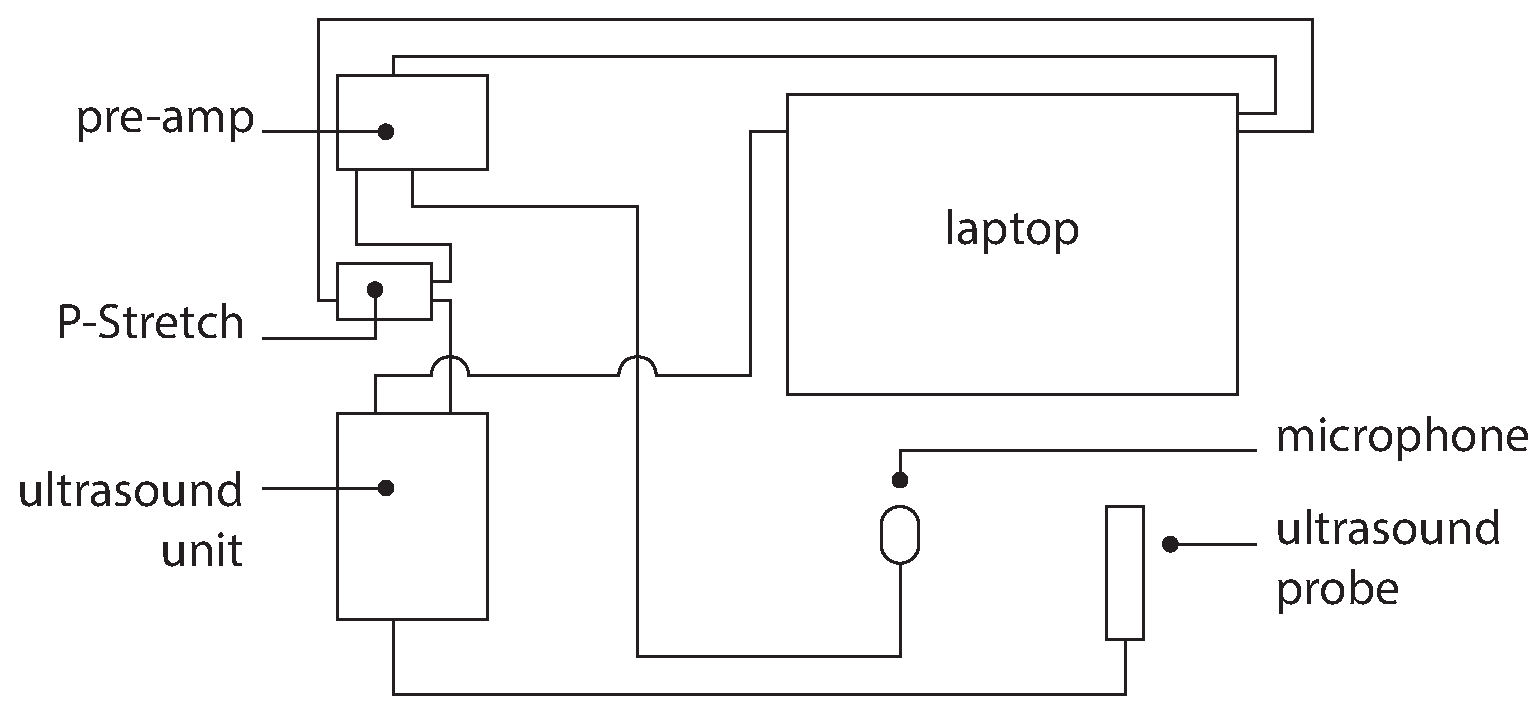
\includegraphics[width=.7\textwidth]{../../graphics/uti-setup.pdf}
    \caption{Schematic representation of the equipment setup (\citealt{articulate2011}, see text for details).}
    \label{f:uti-setup}
\end{figure*}

An Articulate Instruments Ltd™ set-up was used for this study
(\Cref{f:uti-setup}). The ultrasonic data was collected through a
TELEMED Echo Blaster 128 unit with a TELEMED C3.5/20/128Z-3 ultrasonic
transducer (20mm radius, 2-4 MHz). A synchronisation unit (P-Stretch)
was plugged into the Echo Blaster unit and used for automatic
audio/ultrasound synchronisation. A FocusRight pre-amplifier and a Movo
LV4-O2 Lavalier microphone were used for audio recording. The
acquisition of the ultrasonic and audio signals was achieved with the
software Articulate Assistant Advanced (AAA, v2.17.2) running on a
Hawlett-Packard ProBook 6750b laptop with Microsoft Windows 7.
Stabilisation of the ultrasonic transducer was ensured by using a
stabilisation headset produced by Articulate Instruments Ltd™
(\citealt{articulate2008}, not shown in figure).

\subsection{Materials}\label{materials}

Disyllabic words of the form
C\textsubscript{1}V\textsubscript{1}C\textsubscript{2}V\textsubscript{2}
were used as targets, where C\textsubscript{1} = /p/, V\textsubscript{1}
= /a, o, u/, C\textsubscript{2} = /t, d, k, g/, and V\textsubscript{2} =
V\textsubscript{1} (e.g. /pata/, /pada/, /poto/, etc.), yielding a total
of 12 target words. A labial stop was chosen as the first consonant to
reduce influence on the following vowel (although see
\citealt{vazquez-alvarez2007}). Only coronal and velar stops were used
as target consonants since labial consonants cannot be imaged with
ultrasonography. The target words were embedded in a frame sentence.
Prosodically similar sentences were used to ensure comparability between
languages. The frame sentence was \emph{Dico X lentamente} `I say X
slowly' for Italian, and \emph{Mówię X teraz} `I say X now' for Polish.

\subsection{Procedure}\label{procedure}

The sentences with the target words were randomised for each
participant, although the order was kept the same between repetitions
within participant due to software constraints. Each participant
repeated the list of randomised stimuli six times. The participant's
occlusal plane was obtained using a bite plate \citep{scobbie2011}, and
the hard palate was imaged by asking the participant to swallow water
\citep{epstein2005}. The frame rate of the acquisition of the ultrasonic
data ranged between 43 and 68 frames per second. Other settings varied
depending on the frame rate (scanlines = 88-114, pixel per scanline =
980-988, field of view = 71-93, pixel offset = 109-263, depth (mm) =
75-180). The audio signal was recorded at 22050 MHz (16-bit).

\subsection{Data processing and
analysis}\label{data-processing-and-analysis}

Synchronisation of the ultrasonic and audio signal was achieved in
post-processing, using a built-in procedure of AAA. The data were then
subject to force alignment using the SPPAS force aligner
\citep{bigi2015}. The outcome of the automatic annotation was then
manually corrected, according to the criteria in \Cref{t:dur-measures}.
The onset of the target consonant burst (C2 burst) was detected
automatically in Praat \citep{boersma2016}, employing a implementation
of the algorithm described in \citet{ananthapadmanabha2014}. The
durations of the following intervals were extracted from the acoustic
landmarks using an automated procedure in Praat: vowel duration (V1
onset to V1 offset), consonant duration (V1 offset to V2 onset), and
closure duration (V1 offset to C2 burst).

\ctable[caption = List of measurements as extracted from acoustics.,
label = t:dur-measures,
width=\textwidth,
star
]{ll>{\raggedright}p{9cm}}{}{
\FL
\textbf{landmark}               &                  & \textbf{criteria}                                                                                    \ML
vowel onset           & (V1 onset)         & appearance of higher formants in the spectrogram following the burst of /p/ (C1)            \NN
vowel offset          & (V1 offset)        & disappearance of the higher formants in the spectrogram preceding the target consonant (C2) \NN
consonant onset       & (C2 onset)         & corresponds to V1 offset                                                                    \NN
closure onset         & (C2 closure onset) & corresponds to V1 offset                                                                    \NN
consonant offset      & (C2 offset)        & appearance of higher formants of the vowel following C2 (V2); corresponds to V2 onset                                \NN
consonant burst onset & (C2 burst)         & automatic detection \citep{ananthapadmanabha2014}                                           \LL
}

Spline curves were automatically fitted to the visible contours using
the AAA batch tracking function. Manual correction was applied in those
cases that showed clear tracking errors. The time of maximum tongue
displacement within consonant closure was then calculated in AAA
following the method in \citet{strycharczuk2015}. A fan-like frame
consisting of 42 equidistant radial lines was used as the coordinate
system. The origin of the 42 fan-lines coincides with the centre of the
ultrasonic probe, such that each fan-line is parallel to the direction
of the ultrasonic signal. Tongue displacement was thus calculated as the
displacement of the fitted splines along the fan-line vectors. The time
of maximum tongue displacement was the time of greater displacement
along the vector that showed the greatest standard deviation. The vector
search area was restricted to the portion of the splines corresponding
to the tongue tip for coronal consonants, and to the portion
corresponding to the tongue dorsum for velar consonants.

The cartesian coordinates of the tongue contours were exported from two
time points: the onset of C2 closure, and the time maximum tongue
displacement (which is always within C2 closure). The contours were
normalised by applying offsetting and rotation relative to the
participant's occlusal plane \citep{scobbie2011}. Durational
measurements were analysed with linear mixed effects models using
\texttt{lme4} in R \citep{r-core-team2017, bates2015}. Generalised
additive mixed effects regression models \citep[GAMMs,][]{wood2006} were
used for the statistical analysis of tongue contour data.

\section{Results}\label{results}

\subsection{Vowel duration and
voicing}\label{vowel-duration-and-voicing}

A linear mixed effects regression model was fitted to the Italian vowel
duration data with \textsc{duration} as the outcome variable;
\textsc{vowel quality} (/a, o, u/), \textsc{voicing} and
\textsc{place of articulation} of the following consonant,
\textsc{sentence duration} as fixed effects; random intercepts by
speaker and word, and by-speaker random slopes for voicing. An
interaction between voicing and vowel quality was also included in the
final model, since it significantly improved the model. P-values were
obtained with likelihood ratio tests comparing the full model with a
nested model without the tested predictor, and with \texttt{lmerTest}
{[}{]}, which employs the Satterthwaite approximation to degrees of
freedom. According to the full model as specified above, Italian vowels
are 22 milliseconds (SE = 6) longer if followed by a voiced stop
(\(\chi\^2\)(3) = 16.61; p \textless{} 0.001). The following terms and
interactions were also significant: place of articulation C2, vowel
identity, sentence duration, and the interaction between C2 voicing and
vowel identity.

For Polish, the same model structure was used, excluding the
voicing-vowel interaction (which was not significant). Contrary to
previous findings, the model reveals a significant 8 milliseconds effect
(SE = 3) of consonantal voicing on the preceding vowel (\(\chi\^2\)(1) =
5.4, p \textless{} 0.05). Vowel identity and sentence duration were also
significant. The place of C2 significantly improved the model
(\(\chi\^2\)(1) = 6.1, p \textless{} 0.05), so it was included in the
full model even though p \textgreater{} 0.05 according to the single
predictor p-value. The inspection of the model residuals confirmed the
assumptions of normality and homoscedasticity. The exploration of the
random slopes for each speaker indicated that PL05 showed a particularly
higher slope for voicing, meaning that the effect of voicing was
stronger in his data, but removing this speaker from the model doesn't
remove the effect. The estimated effect of voicing on vowel duration for
PL05 was 14 milliseconds. These observations will become relevant when
discussing about the results of the tongue contour data.

\subsection{Tongue contours}\label{tongue-contours}

\label{s:splines}

\begin{figure*}
    \centering
    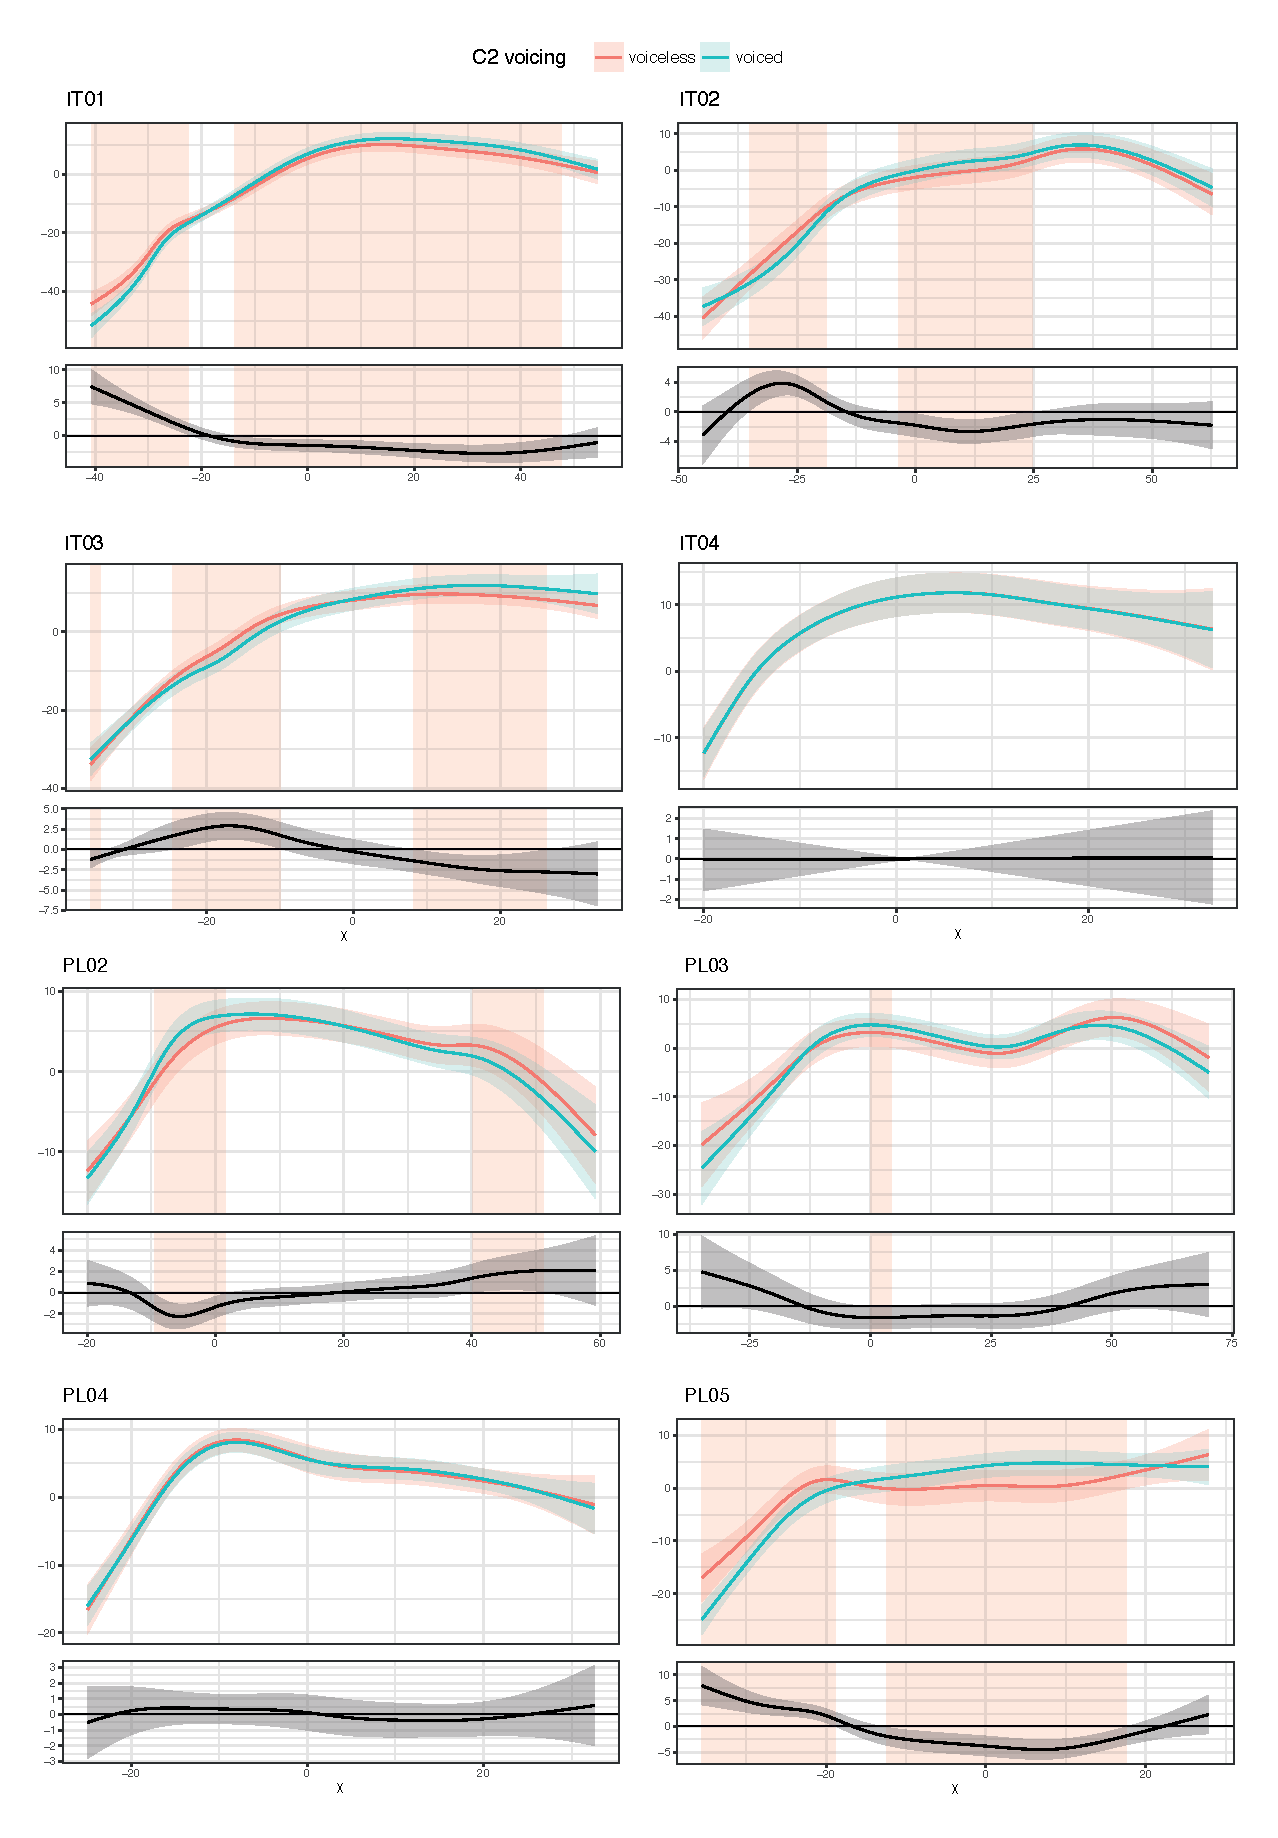
\includegraphics[height=.9\textheight]{fig/tra.pdf}
    \caption{Comparison of tongue contours at maximum tongue displacement (within C2 closure) in Italian (top half) and Polish (bottom half). The plotted contours are reference contours for the coronal consonants preceded by /a/. See \Cref{s:splines} for more details.}
    \label{f:tra}
\end{figure*}

The tongue contour data were analysed with GAMMs \citep{wood2006}.
Individual GAMMs were fitted for each speaker: the
\textsc{y-coordinates} of the contours were included in the model as the
outcome variable; the \textsc{x-coordinates} as the only parametric
term. The following smooths were specified: a reference smooth term for
the x-coordinates, three difference smooths for the x-coordinates by
\textsc{voicing}, \textsc{vowel quality}, and \textsc{place} of
articulation of the following consonant respectively, and
\textsc{by-word} random smooths. A first-order autoregressive model was
included to correct for the high autocorrelation residuals. Significance
testing in GAMMs was achieved through model comparison and visual
inspection of the difference smooth, as suggested in
\citep{soskuthy2017}. Given the poor quality of the ultrasonic data for
/u/, this vowel was not included in the statistical analysis of tongue
contours, hence the results reported in this section only refer to /a/
and /o/.

The analysis of the Italian ultrasonic data shows that voiced stops are
produced with advancement of the root of the tongue, as expected based
on previous research on English. \Cref{f:tra} (top half) shows the
predicted tongue contours in voiceless (dashed line) and voiced stops
(thick line) at maximum tongue displacement for each Italian speaker.
Below each tongue contour panel, the difference smooth for voicing is
also shown (black line, confidence interval in grey). Tongue contours
are significantly different in those point in which the confidence
interval of the difference smooth does not include 0 on the ordinate
axis. The significantly different portions of the contours are also
indicated in the figures by a shaded grey area.

In two participants out of four (IT01, IT02), the root was significantly
more front in voiced stops in both vocalic contexts (/a, o/). On the
other hand, one participant (IT03) had significant tongue root
advancement only following /a/, while the fourth participant (IT04)
didn't show advancement at all. For Polish (bottom half of
\Cref{f:tra}), three out of four speakers (PL02, PL03, PL04) did not
have tongue root advancement, while the fourth speaker (PL05) had
significant advancement in voiced stops in both vocalic contexts.

Further contour analysis was carried out at C2 closure onset for the
Italian and Polish speakers showing advancement. The tongue root at
closure onset was found to be in advanced in voiced consonants ().
Comparisons of tongue contours at C2 onset and at the time of maximum
tongue displacement in voiced consonants further indicated that the
degree of root advancement was larger at maximum displacement for the
Italian speakers (IT01, IT02, IT03), but not for the Polish speaker
(PL05). \Cref{f:voiced} shows the results from IT01 as a representative
example for Italian and from PL05.

\begin{figure*}
    \centering
    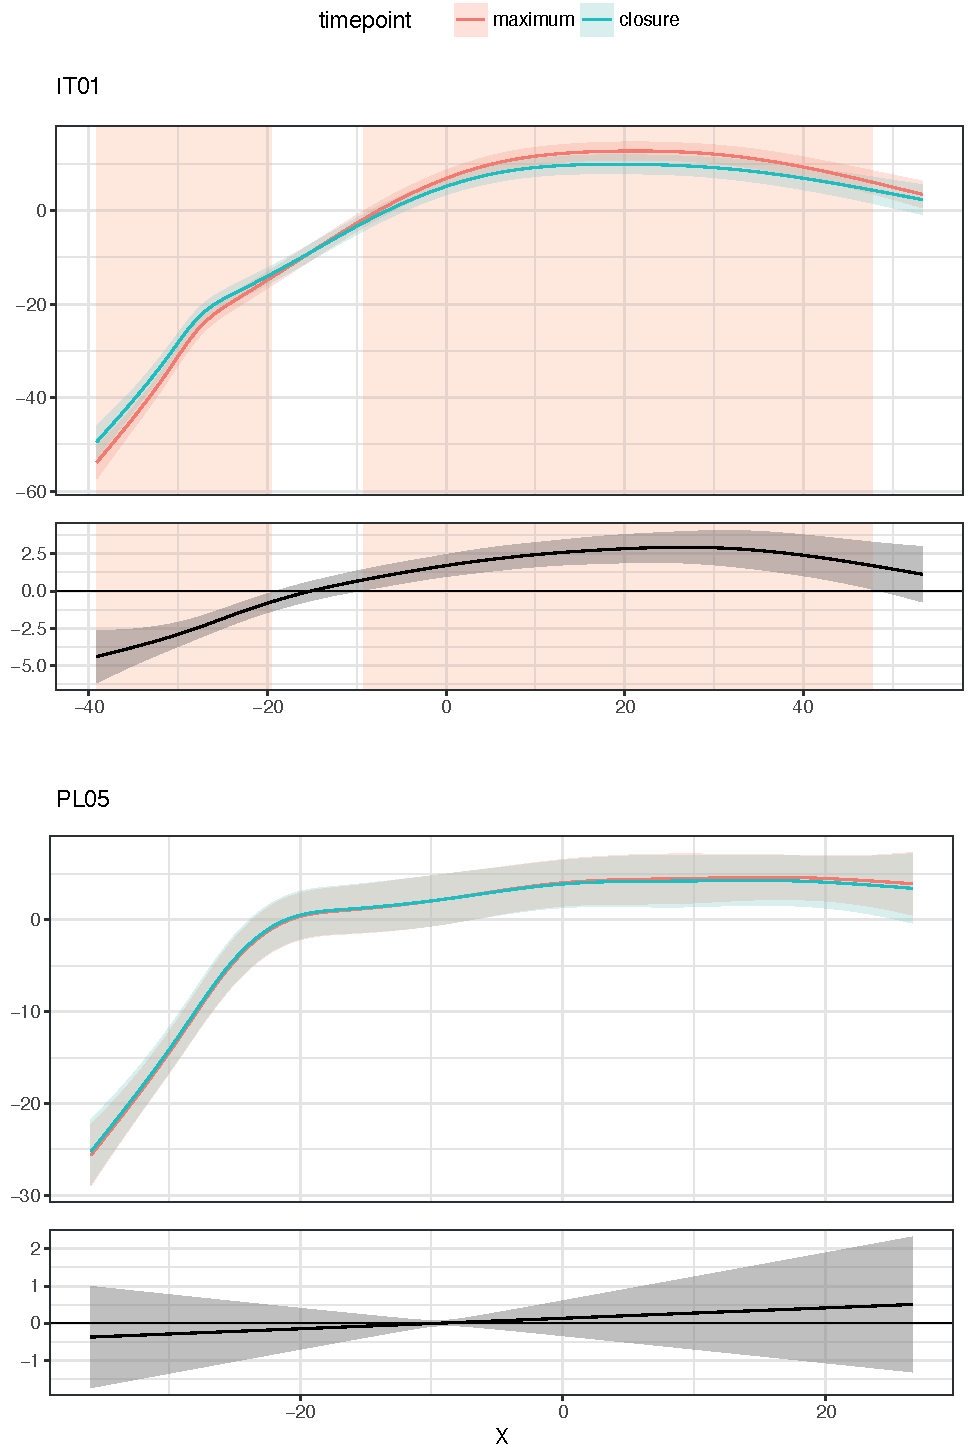
\includegraphics[height=.9\textheight]{fig/voiced.pdf}
    \caption{Comparison of tongue contours of voiced consonants at C2 closure onset and maximum tongue displacement (within C2 closure) in IT01 (Italian) and PL05 (Polish). See text for more details.}
    \label{f:voiced}
\end{figure*}

\section{Discussion}\label{discussion}

\label{s:discussion}

Based on the previously established link between tongue root advancement
and voicing, it was proposed at the beginning of this paper that the
presence of the voicing effect in a language should be correlated with
the presence of tongue root advancement in voiced stops. To test the
correlation between tongue root advancement and vowel durations,
ultrasonic data were collected from two languages that differ in the
presence/absence of the voicing effect, Italian and Polish respectively.
It was predicted that voiced consonants should be produced with an
advanced tongue root in Italian, but not in Polish. However, the results
of this study point to a more fine-grained interpretation of the
proposed link between tongue root and vowel duration.

\begin{figure}
    \centering
    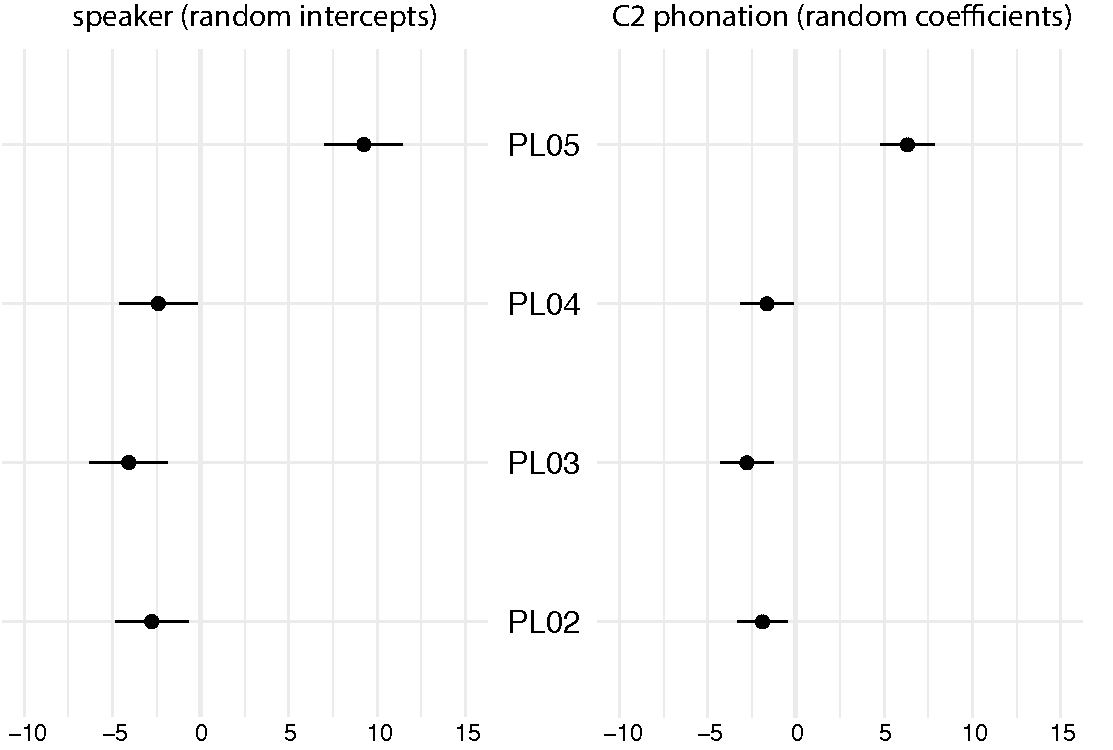
\includegraphics[height=.35\textwidth]{fig/polish-re.pdf}
    \caption{By-speaker random slopes (left) and intercepts (right) for C2 voicing in the Polish vowel duration data. The higher slope estimate for PL05 indicates a relatively stronger effect of voicing on vowel duration for this participant.}
    \label{f:polish-re}
\end{figure}

The durational data of Polish indicate a small effect of voicing in this
language, such that vowels followed by voiced stops are on average 8
milliseconds longer, contrary to previous findings in
\citet{keating1984}. The hypothesis that voiced consonants should not
have tongue root advancement in Polish rests on the assumption that
Polish is a non-voicing-effect language, which does not hold for the
data of this study. The voicing effect was found to be stronger in one
of the Polish speakers, PL05, who has a higher random slope estimate
compared to the other Polish speakers (\Cref{f:polish-re}). Note,
however, that a model fitted to the Polish data with the exclusion of
PL05 still indicates a difference of 6 milliseconds in vowel duration
(\(\chi\^2\)(1) = 8.28; p \textless{} 0.01). Incidentally, though, PL05
is also the only Polish speaker who produced voiced consonants with an
advanced tongue root, both at C2 closure onset and at the time of
maximum tongue displacement.

This pattern is similar to that of the Italian speakers, who have both a
relatively strong voicing effect and tongue root advancement. This is
true for all the speakers of Italian, except one (IT04), whose tongue
root did not differ in voiced and voiceless stops, while still having an
appreciable difference in vowel duration (around 22 milliseconds). A
possible interpretation of the different behaviour of IT04 as an age
effect derives from the older age of this speaker (54 years old, vs an
average of 26 for the other speakers), although a bigger and more
balanced sample is needed for confirmation.

Overall, the speakers who didn't produce voiced consonants with an
advanced tongue root had a relatively weaker voicing effect. On the
other hand, speakers with tongue root advancement showed a relatively
strong effect, with estimates of durational differences ranging between
15 and 30 milliseconds. This generalisation applies independently of the
speaker's language. The fact that the degree of tongue advancement at C2
closure onset and at maximum displacement in the voiced consonants does
not differ in PL05 could be related to the relative weaker effect of
voicing in this speaker. All things considered,

In addition to tongue root advancement, the ultrasonic data also showed
raising of the tongue dorsum. The presence of such gesture, although not
expected, makes sense from an anatomical point of view. Raising of the
tongue body could be implemented as a way to counterbalance the
compression of the tongue mass caused by the advancement of the root. It
is not thus surprising to observe a raised tongue body in voiced stops
accompanying root advancement. An alternative account could ascribe
tongue body raising to aerodynamic properties of voiced stops. Since the
intra-oral pressure is higher in voiced stops due to the amount of air
needed to maintain voicing, a firmer seal at the point of oral
constriction could be used to compensate for the increasing pressure.
Expanding the area of contact by raising the tongue body would provide
for such a firmer constriction.

\section{Conclusion}
\label{s:conclusion}

\bibliography{linguistics.bib}

\end{document}
